\documentclass[UTF8,8pt]{ctexart}
\usepackage{../template/Notes/notes}
\usepackage{multicol}
\setlength{\premulticols}{1pt}
\setlength{\postmulticols}{1pt}
\setlength{\multicolsep}{1pt}
\setlength{\columnsep}{2pt}
\setcounter{secnumdepth}{0}
% Redefine section commands to use less space
\makeatletter
\renewcommand{\section}{\@startsection{section}{1}{0mm}%
    {-1ex plus -.5ex minus -.2ex}%
    {0.5ex plus .2ex}%x
{\normalfont\large\bfseries}}
\renewcommand{\subsection}{\@startsection{subsection}{2}{0mm}%
    {-1explus -.5ex minus -.2ex}%
    {0.5ex plus .2ex}%
{\normalfont\normalsize\bfseries}}
\renewcommand{\subsubsection}{\@startsection{subsubsection}{3}{0mm}%
    {-1ex plus -.5ex minus -.2ex}%
    {1ex plus .2ex}%
{\normalfont\small\bfseries}}
\makeatother
\setlength{\parindent}{0pt}
\setlength{\parskip}{0pt plus 0.4ex}
\geometry{left=0.2cm,right=0.2cm,top=0.3cm,bottom=0.3cm}
\title{Optics Cheatsheet}
\begin{document} 
\leftmargini=5mm
\raggedright
\footnotesize
\begin{multicols}{3}
\begin{comment}
\section{几何光学}
\begin{itemize}  
    \item 光通量$\Phi(lm)=K_{max}\int V\psi \d \l$
    \item 发光强度$I(cd)=\d \Phi/\d \Omega$:点光源单位方位角发出的光通量
    \item 亮度$B(sb)=\d I/\d S$:面光源单位面积发光强度
    \item 照度$E(lx)=\d\Phi/\d S$:照射在单位面积上的光通量。 
    \item 单个折射球面
        $$\f{n'}{s'}+\f{n}{s}=\f{n'-n}{r}$$
        $$V=-\f{ns'}{n's}=-\f{f}{x}=-\f{x'}{f'}\text{(薄透镜也成立)}$$
    \item 反射球面
        $$\ff{s'}+\ff{s}=-\f{2}{r}=\ff{f}$$
        $$V=-\f{s'}{s}$$
    \item 薄透镜
        $$V=-\frac{fs'}{f's}$$ 
        $$\left\{\ar{
            f&=\dfrac{n}{\f{n_L-n}{r_1}+\f{n'-n_L}{r_2}},\\
            f'&=\dfrac{n'}{\f{n_L-n}{r_1}+\f{n'-n_L}{r_2}},\\
        }\right.$$
        当$n = n' \approx 1$:
        $$f=\dfrac{1}{(n_L-1)(\ff{r_1}-\ff{r_2})}$$
    \item 单个厚透镜
        \putfig{0.35}{1.png}
        $$\text{光焦度}P=(n-1)(\frac{1}{r_1}-\frac{1}{r_2})+\frac{(n-1)^2}{nr_1r_2}d $$
        $$\rightarrow (n-1)(\frac{1}{r_1}-\frac{1}{r_2})$$
        $$a=\frac{(n-1)d(r_2-r_1+d)}{n(r_2-r_1)+(n-1)d} \rightarrow \f{(n-1)d}{n}$$
        $$l_H=\frac{r_1d}{n(r_2-r_1)+(n-1)d} \rightarrow \frac{r_1d}{n(r_2-r_1)}$$
        $$l_H'=\frac{r_2d}{n(r_2-r_1)+(n-1)d} \rightarrow \frac{r_2d}{n(r_2-r_1)}$$
    \item 拉格朗日-亥姆霍兹定理:
        设$u$为光线与光轴夹角,$y$为像高,
        $$ynu=y'n'u'$$
    \item 密接透镜
        $$P=\sum P_i$$
    \item 理想光具组
        \putfig{0.25}{2.png}
        $$f=\f{f_1f_2}{\Delta}\ \ f'=-\f{f_1'f_2'}{\Delta}$$
        $$x_F=\f{f_1f_1'}{\Delta}\ \ x_F'=-\f{f_2f_2'}{\Delta}$$
        $$l_F=-f'(1+\f{d}{f_2})\ \ l_F'=f'(1-\f{d}{f_1'})$$
        $$l_H=-\f{d}{f_2}f'\ \ l_H'=-\f{d}{f_1'}f'$$
    \item 视角放大率\\
        放大镜($s_0=25cm$)
            \putfig{0.3}{3.png}
            $$M=\f{s_0}{f}$$
        显微镜($f_O$物镜,$f_E$目镜)
            \putfig{0.3}{4.png}
            $$M=-\f{s_0\Delta}{f_Of_E}$$
        望远镜
            \putfig{0.3}{5.png}
            $$M=-\f{f_O}{f_E}$$
    \item 色差
    令$K_1=\ff{r_1}-\ff{r_2},\ K_2=\ff{r_2}-\ff{r_3}$,消色差时
    $$P_F-P_C=(n_{1F}-n_{1C})K_1+(n_{2F}-n_{2C})K_2=0$$

\end{itemize}
\se{干涉}    
\begin{itemize}
    \item 杨氏双缝
        $$\delta=-\f{2\pi d}{\l D}x$$
        $$\Delta x=\f{\l D}{d}$$
    \item 杨氏双缝条纹位移与点源位移关系:
        $$\delta x=-\f{D}{R}\delta s$$
    \item 空间相干性:当$\delta x=\Delta x$时为极限光源宽度
        $$b_0=\f{R}{d}\l \approx \f{\l}{\delta\t}$$
    \item 等厚干涉
        相邻条纹厚度差:
        $$\Delta h=\f{\l}{2n}$$
    \item 牛顿环$k$级暗纹半径$r_k$与曲率半径$R$关系
        $$r_k=\sqrt{kR\l},\quad R=\f{r^2_{k+m}-r^2_k}{m\l}$$
    \item 增透膜 
        $$n=\sqrt{n_1n_2}$$
    \item 等倾条纹
        $$\Delta L=2nh\cos i,\quad h,i\text{为膜厚度,反射角}$$
        $$\Delta r \propto -\f{\l}{2nh\sin i_k}$$
    \item 迈克尔逊干涉仪
            $$I=I_0(1+\cos\delta),\quad \delta=k\Delta L$$
    \item 双线光源衬比度
        $$\gamma=\left|\cos(\D k\D L/2)\right|$$
        当移动$\D L=\f{\l^2}{2\D\l}$时,衬比度第一次降为0.
    \item 连续谱光源衬比度
        $$\gamma=\left|\f{\sin(\D k\D L/2)}{\D k\D L/2}\right|$$
        当移动$\D L_{max}=\f{\l^2}{\D\l}$时,衬比度第一次降为0.这也是一个波列的长度。
    \item 相干长度
        $$L_0=\D L_{max}=\f{\l^2}{\D\l}$$
    \item 多光束干涉,薄膜两侧$n$相等时,有斯托克斯关系:
        $$r=-r',\quad r^2+tt'=1$$
    \item 多光束干涉,透射反射光强:
        $$U_T=\f{Att'}{1-r^2e^{i\delta}}$$
        $$I_T=\dfrac{I_0}{1+\f{4R\sin^2(\delta/2)}{(1-R)^2}}$$
        $$I_R=I_0-I_T=\dfrac{I_0}{1+\f{(1-R)^2}{4R\sin^2(\delta/2)}}$$
    \item F-P干涉 半峰宽$\varepsilon$
        $$\varepsilon=\f{2(1-R)}{\sqrt{R}}$$
    \item F-P干涉,单色光,$\delta=4\pi n h\cos i/\l$, 取$\varepsilon=d\delta,i=i_k$可得$k$级亮纹角宽度
        $$|\D i_k|=\f{\l}{2\pi nh\sin i_k}\f{1-R}{\sqrt{R}}$$
        这说明腔长$h$越长,条纹越细锐。
    \item F-P干涉,复色光,$2nh=k\l,\quad k \in \mathbb{Z}$,$\nu$称为纵模,则纵模间隔:
        $$\D\nu=\f{c}{2nh}$$
        在某一点只有相距$\D\nu$的光在该点极大。\\
        纵模宽度为:
        $$\D\l_k=\f{\l}{\pi k}\f{1-R}{\sqrt{R}}$$
        $$\D\nu_k=\f{c\D\l}{\l^2}=\f{c}{\pi k\l}\f{1-R}{\sqrt{R}}$$
\end{itemize}
\end{comment} 
\se{4 衍射}
\begin{itemize}
\sub{4.1}
\item 惠更斯-菲涅尔原理:波前$\Sigma$上每个面源$\d\Sigma$都可以看成新的振动中心,它们发出次波。在空间某一点$P$的振动是所有次波在该点的相干叠加。
\item 菲涅尔-基尔霍夫衍射积分公式:
    \putfig{0.1}{6.jpg}
    $$\widetilde{U}(P)=\f{-i}{2\l}\iint{(\cos\t_0+\cos\t)\widetilde{U}_0(Q)\f{e^{ikr}}{r}\d\Sigma}$$
    傍轴条件下:
    $$\widetilde{U}(P)=\f{-i}{\l r_0}\iint{\widetilde{U}_0(Q)e^{ikr}\d\Sigma}$$
\sub{4.2}
\item 半波带法
    $$A(P_0)=\ff{2}(A_1+(-1)^{n+1}A_n)$$
    波带半径$\rho_k=\sqrt{\f{Rb}{R+b}k\l}=\sqrt{k}\rho_1$
    $$\ff{f}=\f{k\l}{\rho_k^2}=\ff{R}+\ff{b}$$
    次焦点$f'=\pm \f{2k+1}f$
\sub{4.3}
\item 单缝夫琅禾费衍射($I_0$为场中心强度,$a$为缝宽度, $\a=\f{\pi a}{\l}\sin\t$)
    $$I_\t=I_0(\f{\sin\a}{\a})^2$$ 
\item 暗纹位置
    $$\sin\t=\pm\f{\l}{a},\ \a=\pm n\pi$$
\item 亮斑角宽度=零级亮斑半角宽
    $$\D\t=\f{\l}{a}$$
\item 圆孔夫琅禾费衍射,$a$为半径,$(x=\f{2\pi a}{\l}\sin\t)$
    $$I(\t)=I_0\left[\f{2J_1(x)}{x}\right]^2$$
\sub{4.4}
\item 艾里斑
    $$\D\t=0.61\f{l}{a}=1.22\f{\l}{D}$$
\item  判断最小分辨角的瑞利判据:
    $$\delta \t_{min}=1.22\f{\l}{D}$$
\item 最小分辨距离($u$为透镜半径/物距夹角),截止频率的倒数即为分辨距离
    $$\de y_{min}=\f{0.61\l}{n\sin u}$$
\sub{4.5}
\item 光栅强度分布($d$为光栅常数)
    $$I=a_0^2(\f{\sin\a}{\a})^2(\f{\sin N\beta}{\sin\beta})^2,$$
    $$\a=\f{\pi a}{\l}\sin\t,\ \beta=\f{\pi d}{\l}\sin\t$$
\item 光栅主极大
    $$\sin\t=k\f{\l}{d}$$
\item 光栅零点(相邻$k$有$N-1$条)
    $$\sin\t=(k+\f{m}{N})\f{\l}{d},m=[1,N-1]$$
\item 光栅半角宽
    $$\D\t=\f{\l}{Nd\cos\t_k} \approx \f{\l}{Nd}$$
\item 正弦光栅(仅有三个主极大)
    $$\widetilde{U} \propto \f{\sin\beta}{\beta}+\ff{2}\f{\sin(\beta-\pi)}{\beta-\pi}+\ff{2}\f{\sin(\beta+\pi)}{\beta+\pi}$$
\sub{4.6}
\item 角/线色散本领
    $$D_l=\f{\de l}{\de\l}=fD_\t=f\f{\de \t}{\de\l}=f\f{k}{d\cos\t_k}$$ 
\item 色分辨本领
    $$R =\equiv \f{\l}{\de\l}=kN$$
\item 工作波段限制
    $$\l_{max}<d,\ \l_{min}>\l_{max}/2$$
\item 闪耀光栅$n$级闪耀波长
    $$2d\sin\t_b=n\l_{2b}$$
\end{itemize}
\se{5 变换光学与全息成像}
\begin{itemize}
\sub{5.1}
    \item 平面波前函数
    $$U(x,y)=U(O)\exp(ik(\sin\t_1 x+\sin\t_2y)),$$
    $$\qquad U(O)=Ae^{i\phi(O)}$$
    \item 球面波前函数(指数+则发散)
    $$U=A/\sqrt{(x-x_0)^2+(y-y_0)^2+z^2}$$
    $$\times \exp(\pm ik\sqrt{(x-x_0)^2+(y-y_0)^2+z^2})$$
    \item 傍轴球面波前函数\\
        $U=$
        $$\f{Ae^{ikr_0}}{z}\exp(ik\f{x^2+y^2}{2z})\exp(-ik\f{xx_0+yy_0}{z})$$
    \item 远场球面波前函数\\
        $U=$
        $$\f{Ae^{ikz}}{z}\exp(ik\f{x^2+y^2}{2z})\exp(-ik\f{xx_0+yy_0}{z})$$
    \item 透镜相位变换函数(屛函数)
        $$T=\exp(-ik\f{x^2+y^2}{2F})$$
    \item 楔形棱镜\\
    $T=\exp(-ik(n-1)\a x)$,$\a$楔角,$n$折射率
\sub{5.2}
    \item 空间频谱,$1/d$为(物)空间频率
        $$\sin\t_n=n\l/d$$
        $$T=\f{a}{d}\f{\sin\a_n}{\a_n},\ \a_n=n\pi a/d$$
    \item 相干光分辨本领:以孔径能传递0、1级谱为条件
        $$\f{D/2}{f} \leq \sin\t=\f{\l}{d}$$
    \item 阿贝成像原理\\
        1. 物平面发出夫琅禾费衍射,在透镜像方焦面上形成衍射图样是物平面的空间频谱。\\
        2. 频谱面上的各衍射斑发出的次波在像平面上干涉,形成的图样即为像。
    \item 空间滤波实验\\
        在频谱面上加滤波器改变频谱,以修饰或改变像。
    \item 相称显微镜\\
        在显微镜物镜的后焦面上加空间滤波器滤掉低频,可将相位型的物变成有衬度的振幅型。
        $$I=A_1^2[3+2\cos\de+2\phi\sin\de-2\cos\de-2]$$
        $$=A_1^2[1+2\phi\sin\de]$$
        反衬度取决于$2\phi\sin\de, \de=\pm \f{\pi}{2}$反衬度最大
    \item 相称显微镜
\sub{5.3}
    \item 夫琅禾费衍射装置\\
        标准远场:
        $$U=Ae^{ikr_0}$$
        $$\cdot\iint T\exp(-ik(\sin\t_1 x+\sin\t_2y))\d x\d y$$
        远场接收:
        $$U=Ae^{ikz}\exp(ik\f{x'^2+y'^2}{2z})$$
        $$\cdot\iint T\exp(-ik\f{xx'+yy'}{z})\d x\d y$$
        焦面接收:
        $$U=Ae^{i\phi}$$
        $$\cdot\iint T\exp(-ik(\sin\t_1 x+\sin\t_2y))\d x\d y$$
        像面接收:
        $$U=A\exp(ik(SQS'))\exp(ik\f{x'^2+y'^2}{2z})$$
        $$\cdot\iint T\exp(-ik(\sin\t_1 x+\sin\t_2y))\d x\d y$$
\sub{5.4}
    \item 全息照相:无源空间的边值定解\\
        1. 物光波+参考光波=物光波前的全息记录(全息图)\\
        2. 照明波+全息图=物光波前的重建(+1级虚像,-1级实像(凹凸反转))
    \item 体全息\\
        介质中纵深条纹记录,再现时三维衍射。
    \item 应用\\
        全息电影,全息电视,全息显微技术,全息干涉技术。
\end{itemize}
\se{6 偏振}
\begin{itemize}
\sub{6.1}
    \item 旋光方向\\
    波垂直于纸面迎面而来,若$E$按逆时针旋转则为左旋光。
    \item 马吕斯定律
        $$I_2=A_2^2=I_1\cos^2\t$$
    \item 偏振度
    $$P=\f{I_{max}-I_{min}}{I_{max}+I_{min}}$$
\sub{6.2}
    \item{各种反射率}
    $$\begin{array}{l|c|c}
        &p\text{分量}&s\text{分量}\\
        \text{振幅反射率}r&E'_{1p}/E_{1p}&E'_{1s}/E_{1s}\\
        \text{强度反射率}R&r_p^2&r_s^2\\
        \text{能流反射率}R'&r_p^2&r_s^2\\
        \text{振幅透射率}t&E'_{2p}/E_{1p}&E'_{2s}/E_{1s}\\
        \text{强度透射率}T&\f{n_2}{n_1}|t_p|^2&\f{n_2}{n_1}|t_s|^2\\
        \text{能流透射率}T'&\f{\cos i_2}{\cos i_1}T_p & \f{\cos i_2}{\cos i_1}T_s
    \end{array}$$
    \item 光的强度
    $$I=\f{n}{2c\mu_0}|E|^2 \propto n|E|^2$$
    \item 各种守恒
    $$\begin{array}{r|r}
        R_p+\f{\cos i_2}{\cos i_1}T_p=1&R_s+\f{\cos i_2}{\cos i_1}T_s=1\\
        |r_p|^2+\f{n_2\cos i_2}{n_1\cos i_1}|t_p|^2=1&|r_s|^2+\f{n_2\cos i_2}{n_1\cos i_1}|t_s|^2=1\\
        r^2+tt'=1&r'=-r
    \end{array}$$
    \item 菲涅尔公式
    $$\ar{
        E'_{1p}=\f{n_2\cos i_1-n_1\cos i_2}{n_2\cos i_1+n_1\cos i_2}E_{1p}&=\f{\tan(i_1-i_2)}{\tan(i_1+i_2)}E_{1p}\\
        E_{2p}=\f{2n_1\cos i_1}{n_2\cos i_1+n_1\cos i_2}E_{1p}\\
        E'_{1s}=\f{n_1\cos i_1-n_2\cos i_2}{n_1\cos i_1+n_2\cos i_2}E_{1s}&=\f{\sin(i_2-i_1)}{\sin(i_2+i_1)}E_{1s}\\
        E_{2s}=\f{2n_1\cos i_1}{n_1\cos i_1+n_2\cos i_2}E_{1s}&=\f{2\cos i_1\sin i_2}{\sin(i_1+i_2)}
    }$$
    \item 布鲁斯特角=入射角的$p$方向反射率为0
    $$i_B=\arctan(n_2/n_1)$$
    \item 半波损失
    
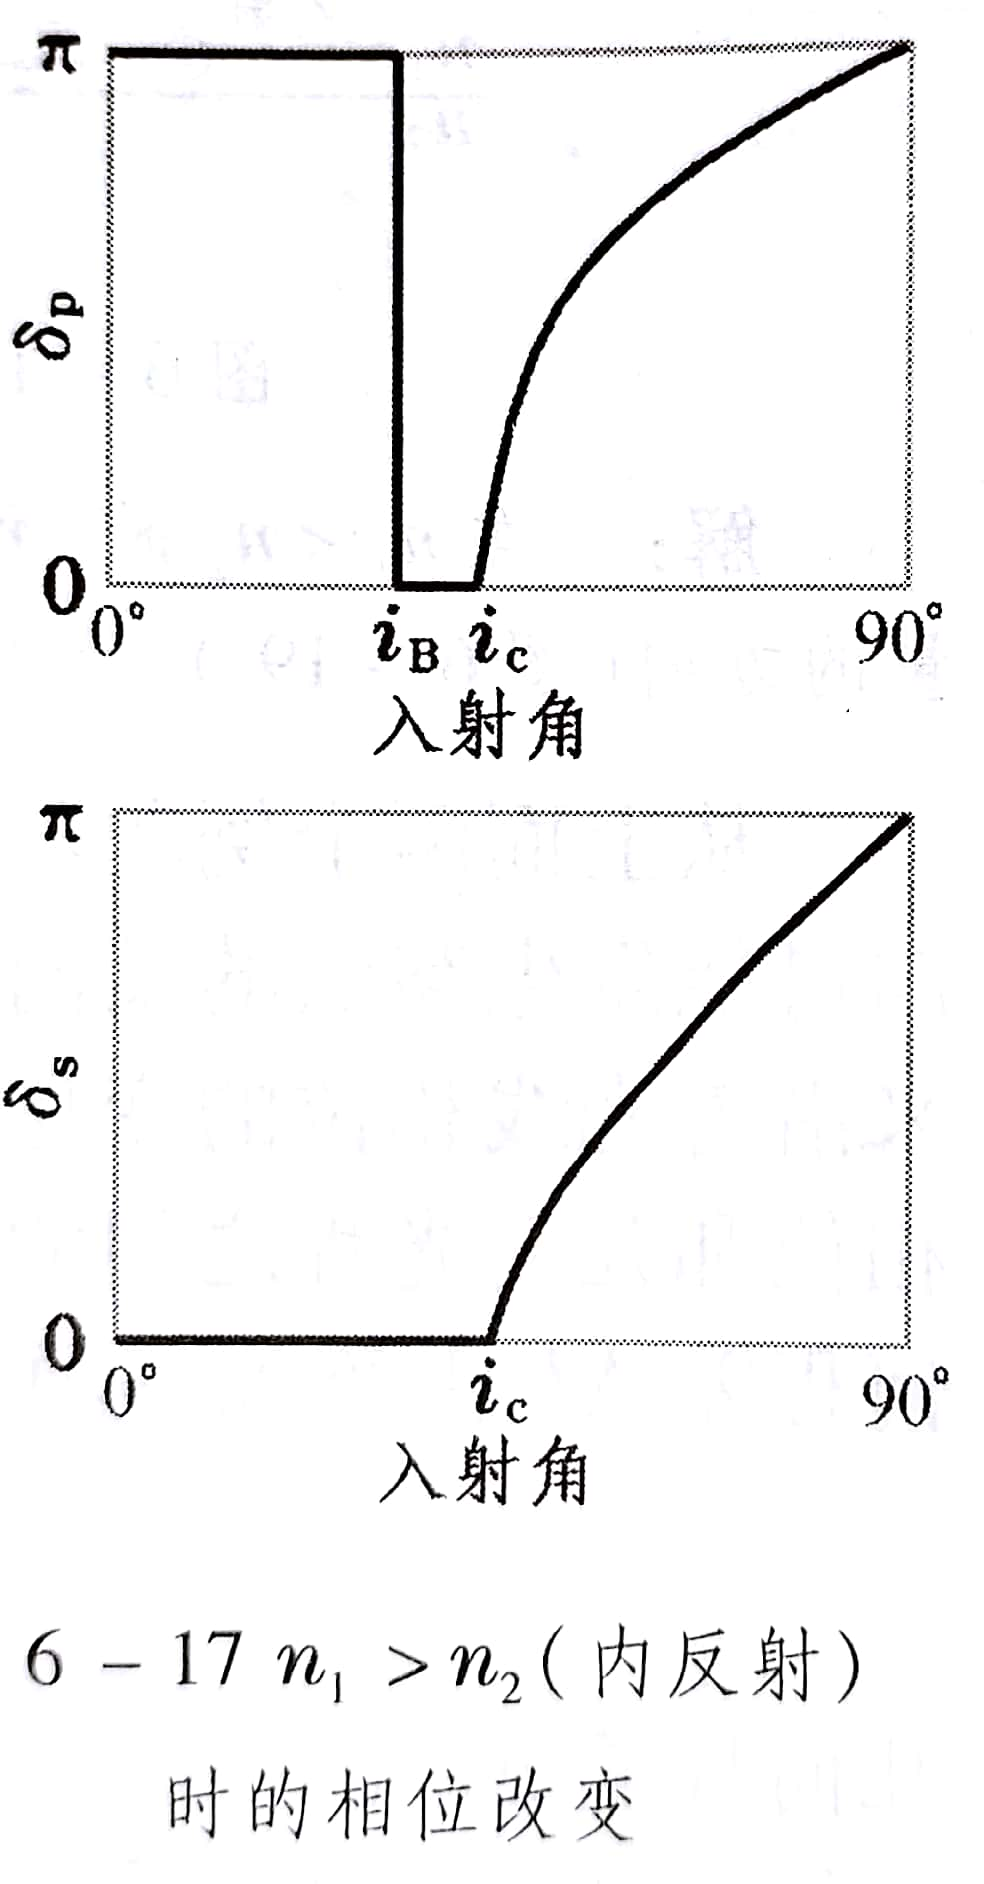
\includegraphics[scale=0.06]{11.jpg}
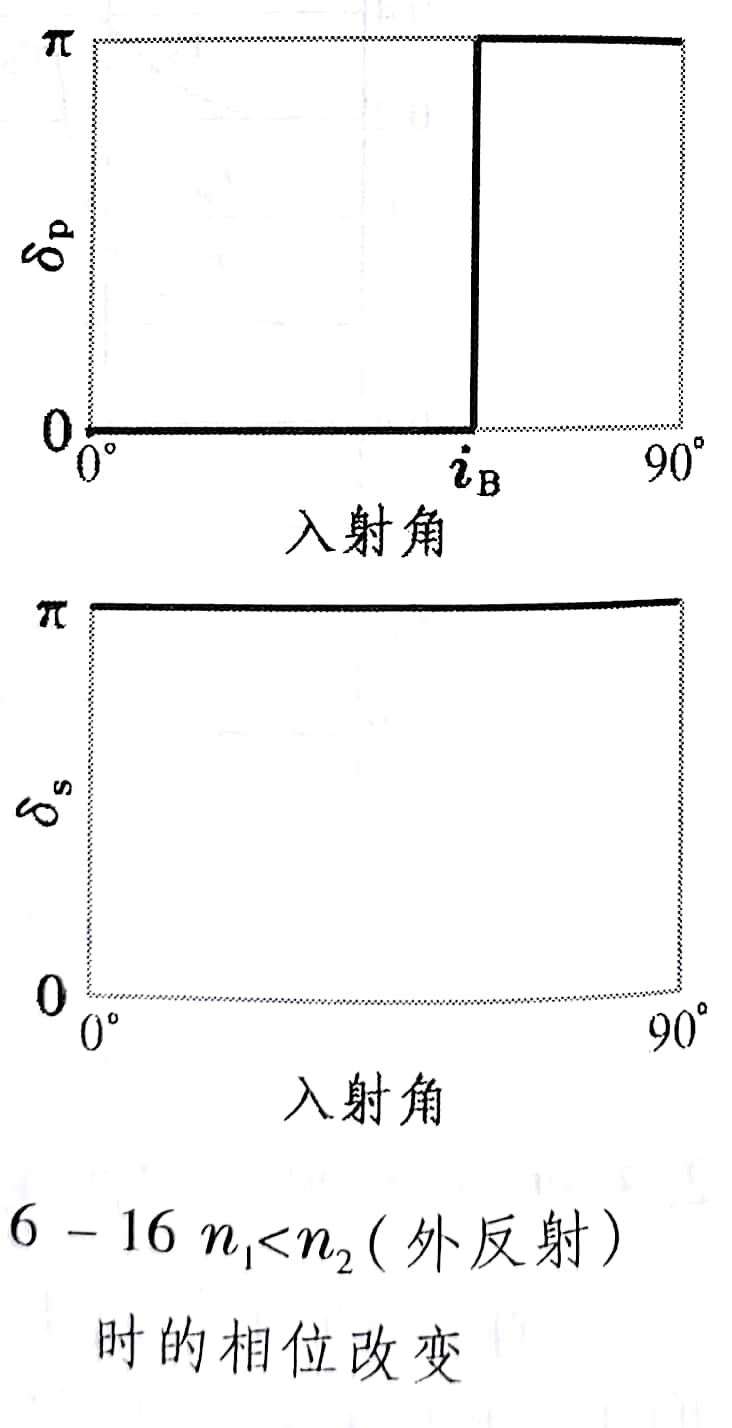
\includegraphics[scale=0.08]{12.jpg}
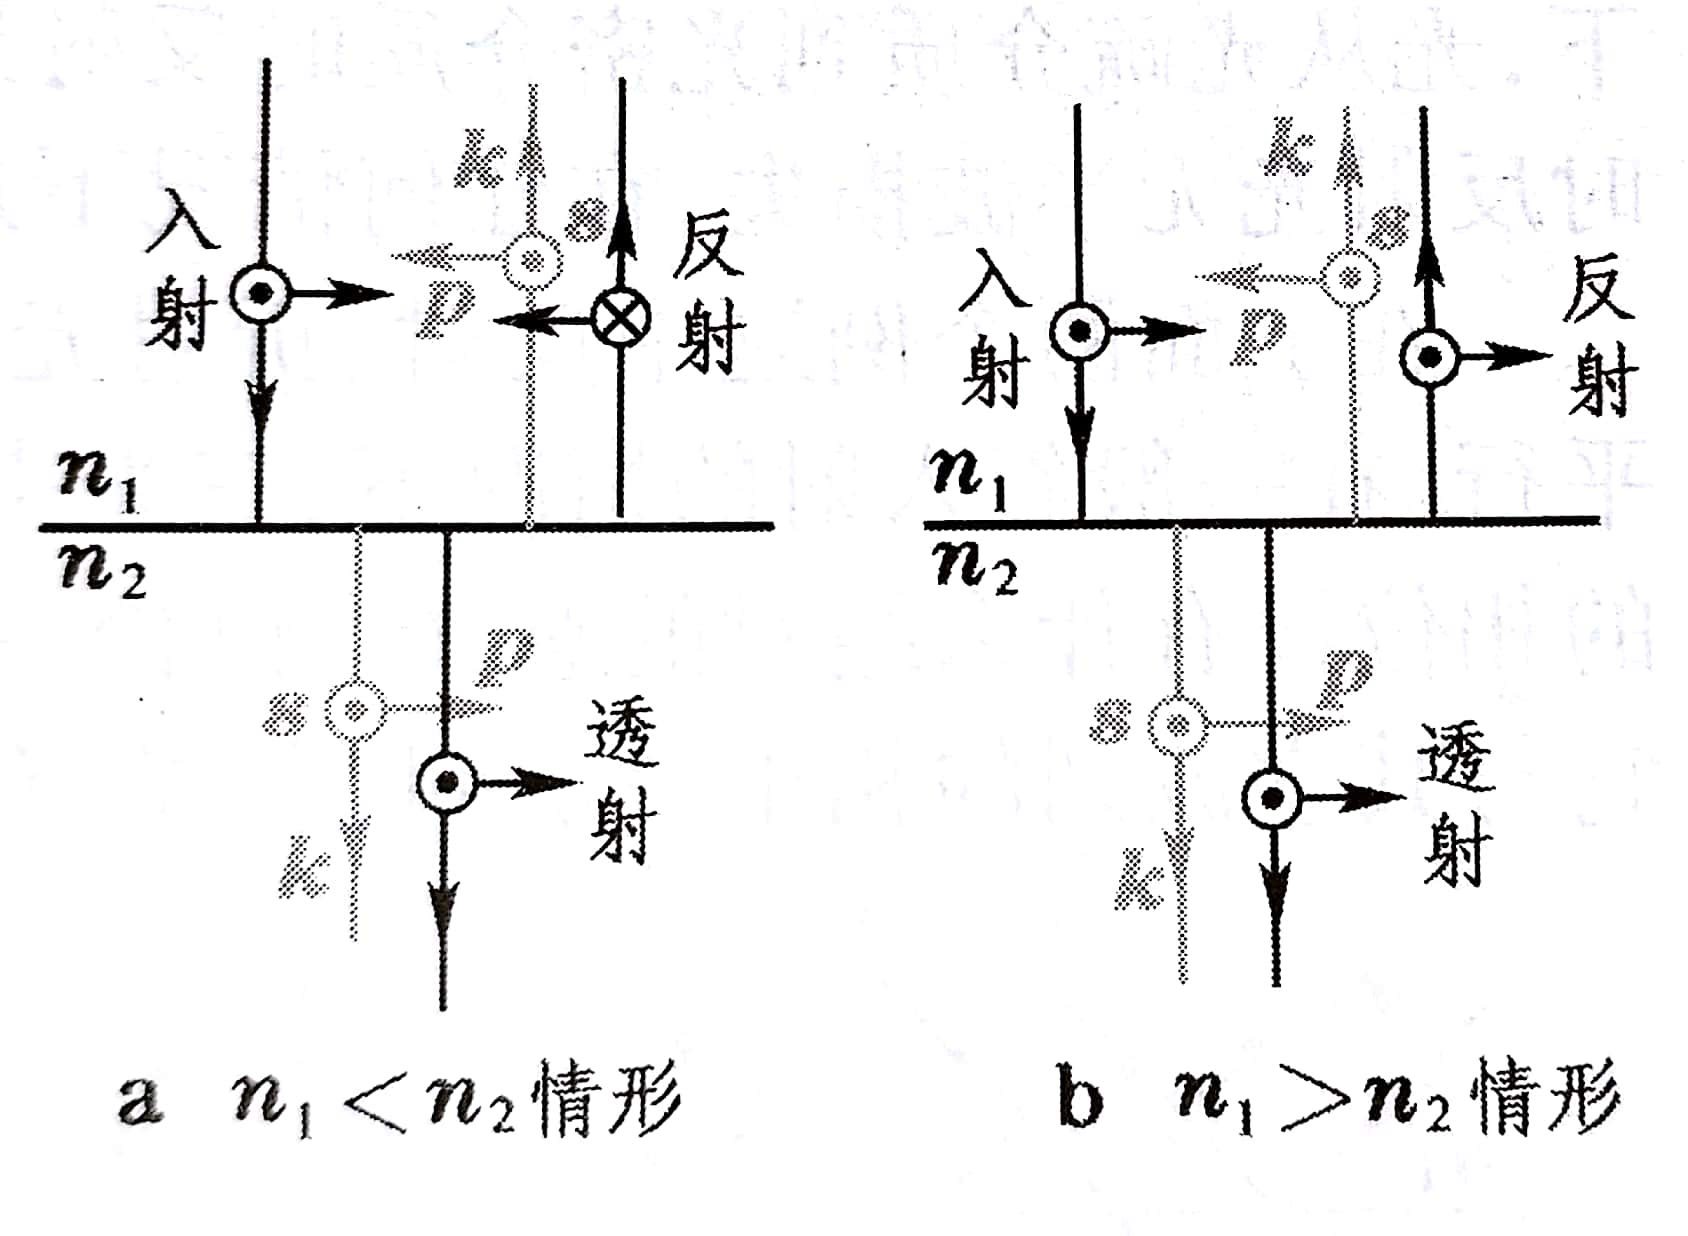
\includegraphics[scale=0.07]{13.jpg}
\sub{6.3}
    \item 寻常光(o光)-垂直方向
    \item 非常光(e光)-平行方向
    \item 光轴方向o,e光不分开, 对角线方向。
    \item 主截面,与光轴垂直的平面。若主截面与入射面重合,则两折射线皆在入射面内。
    \item 负晶体-冰洲石-$v_e>v_o$,正晶体-石英-$v_o>v_e$
\sub{6.4}
\item 晶体偏振器
    \putfig{0.05}{7.jpg}
    \putfig{0.05}{8.jpg}
\item 波晶片\\
相位差$\D\phi=\f{2\pi}{\l}\D l=\f{2\pi}{\l}(n_o-n_e)d$
\item 偏振光经过$\l/4$片后变化
\begin{center}
    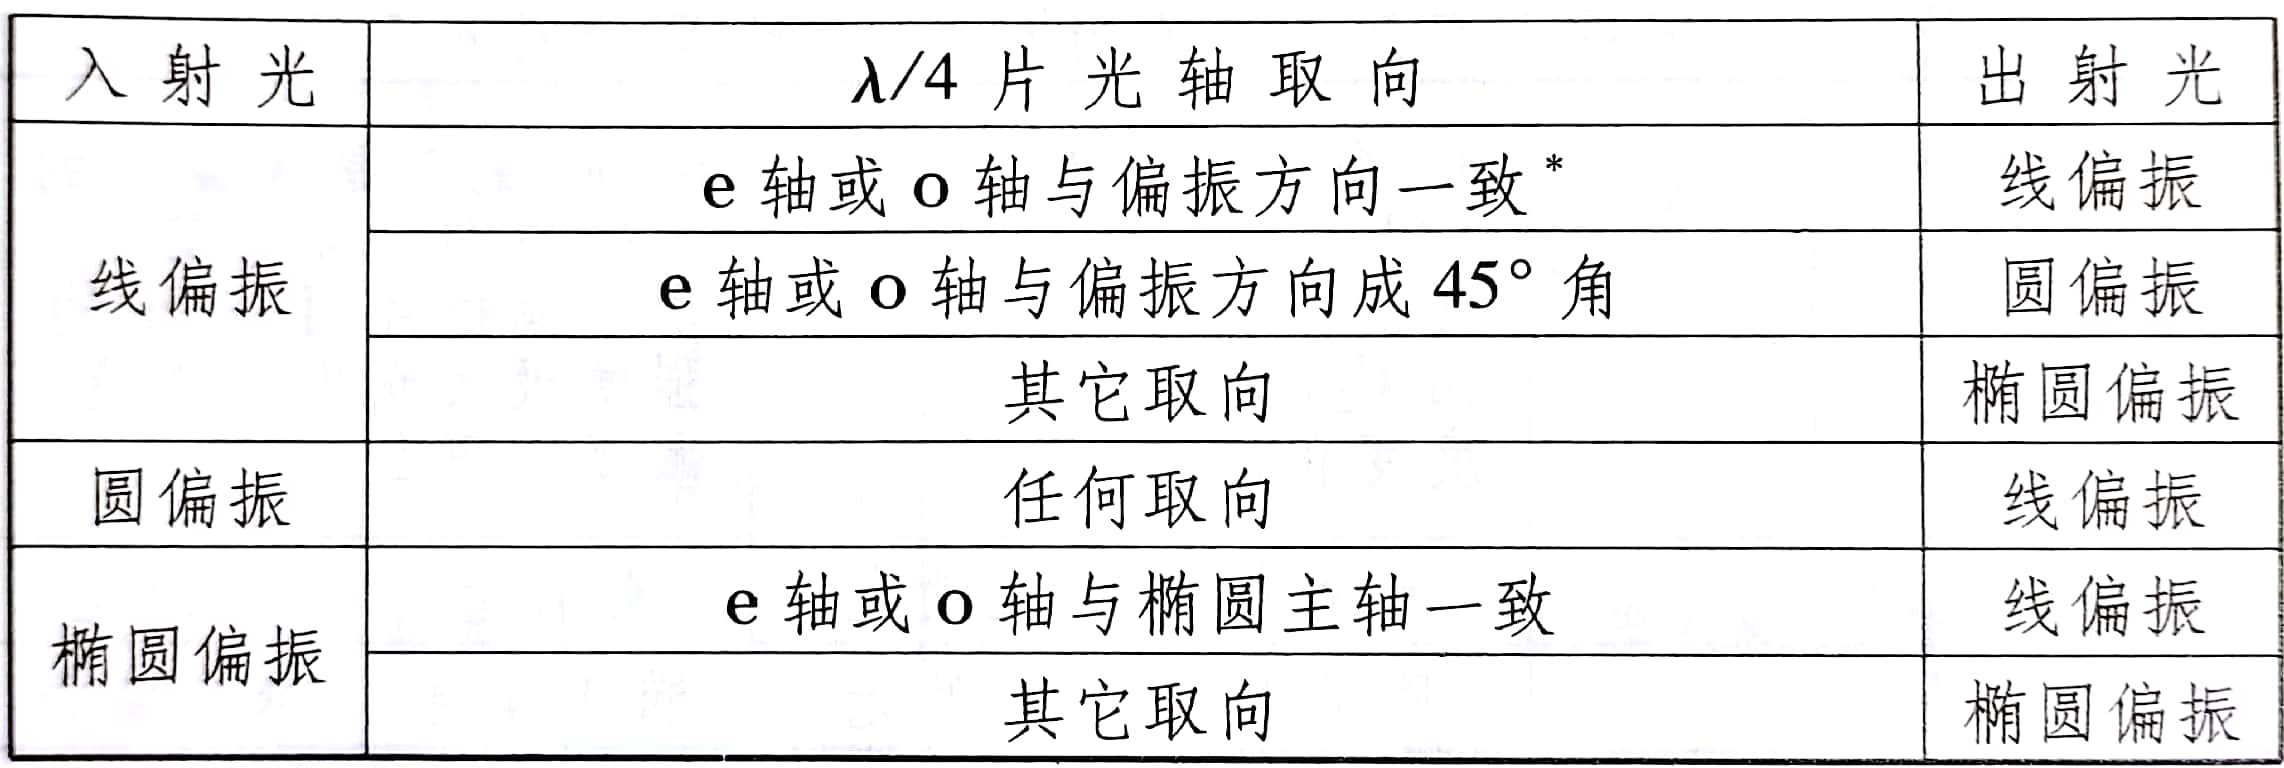
\includegraphics[scale=0.1,angle=270]{9.jpg}
\end{center}
\item 偏振光检验
\begin{center}
    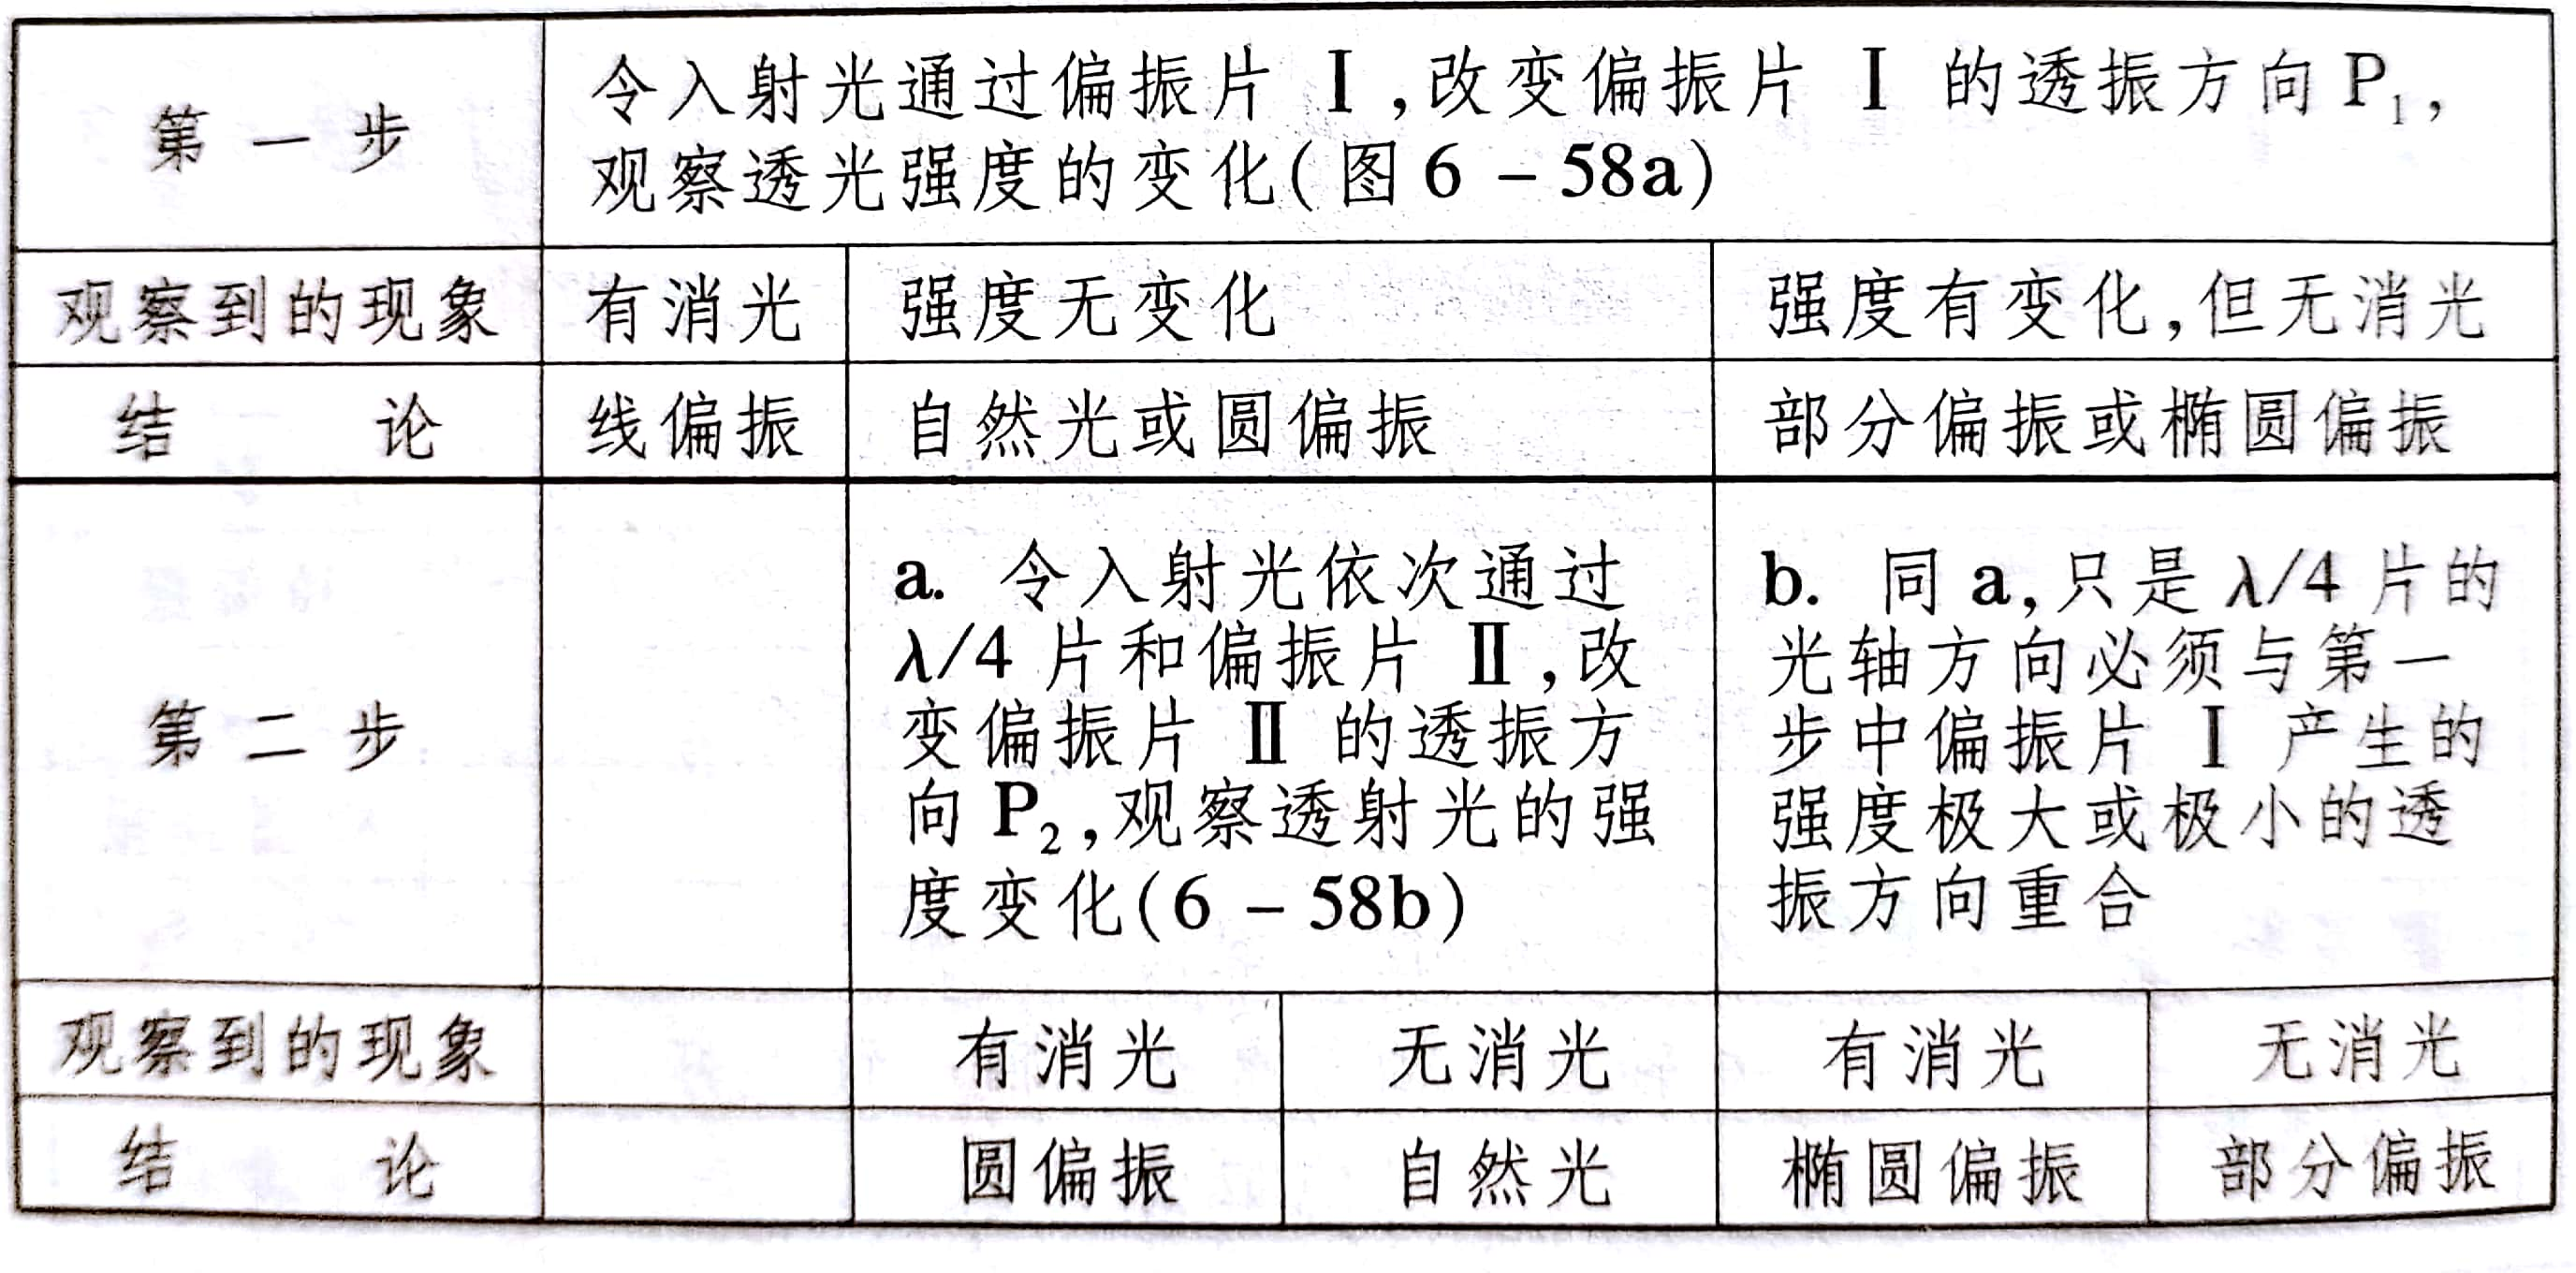
\includegraphics[scale=0.1,angle=270]{10.jpg}
\end{center}
\sub{6.5}
\item 当(1) $P_1 \perp P_2,e$轴为角平分线,(2) $P_1,e$轴不动,$P_2$转到与$P_1$平行。
$$\ar{
    P_1 \perp P_2,I_2=&\f{A_1^2}{2}[1+\cos(\D+\pi)]\\
    =&\f{A_1^2}{2}(1-\cos\D)\\
    P_1 \parallel P_2,I_2=&\f{A_1^2}{2}(1+\cos\D)
}$$
\end{itemize}
\se{7 光与物质相互作用 光的量子性}
\begin{itemize}
    \sub{7.1}
    \item 吸收系数/布格定律
    $$-\d I=\a I\d x$$
    $$I=I_0e^{-\a l}$$
    $a^{-1}$的意义是光减少到原来的$e^{-1} \approx 36\%$所需要的厚度。
    \item 比尔定律:对于溶液,其吸收系数与浓度成正比:
    $$\a=AC \ip I=I_0e^{-ACl}$$
    \item 复数折射率,衰减指数
    $$\a=2n\kappa\o /c=4\pi n\kappa /\l$$
    $$\widetilde{n}=n(1+i\kappa),\ \widetilde{E}=E_0\exp(-i\o(t-nx/c))$$
    \item 光谱:\\
    原子气体-线光谱\\
    分子-带光谱
    \sub{7.2}
    \item 正常色散:\\
    $n$随$\l$增大而下降,且下降率在短波一端更大。
    \item 柯西正常色散经验公式:
    $$n=A+\f{B}{\l^2}+\f{C}{\l^4}$$
    \item 相速$v_p$:波面传播速度,折射率法测。
    $$v_p=\f{c}{n}$$
    \item 群速$v_g$:波包振幅最大的地方的传播速度
    $$v_g=\dd{\o}{k}$$
    \item 群速与相速关系
    $$\f{c}{v_g}=\f{c}{v_p}+\o\dd{n}{\o} \ip n_g=n-\l\dd{n}{\l}$$
    当$\dd{n}{\l}<0$, 群速小。
\end{itemize}
\end{multicols}
\end{document}